\section{Power and Energy Consumption}
\noindent

\subsection{Power analysis}
The available data spans in the range of April 2020 to October 2022. 
The fluctuations of data do not demonstrate the pattern of seasonality visually, which is further confirmed with the STL analysis tool (Figure \ref{fig:PWR_STL}), which also did not demonstrate the seasonality pattern of energy consumption.

\begin{figure}[H]
    \centering
    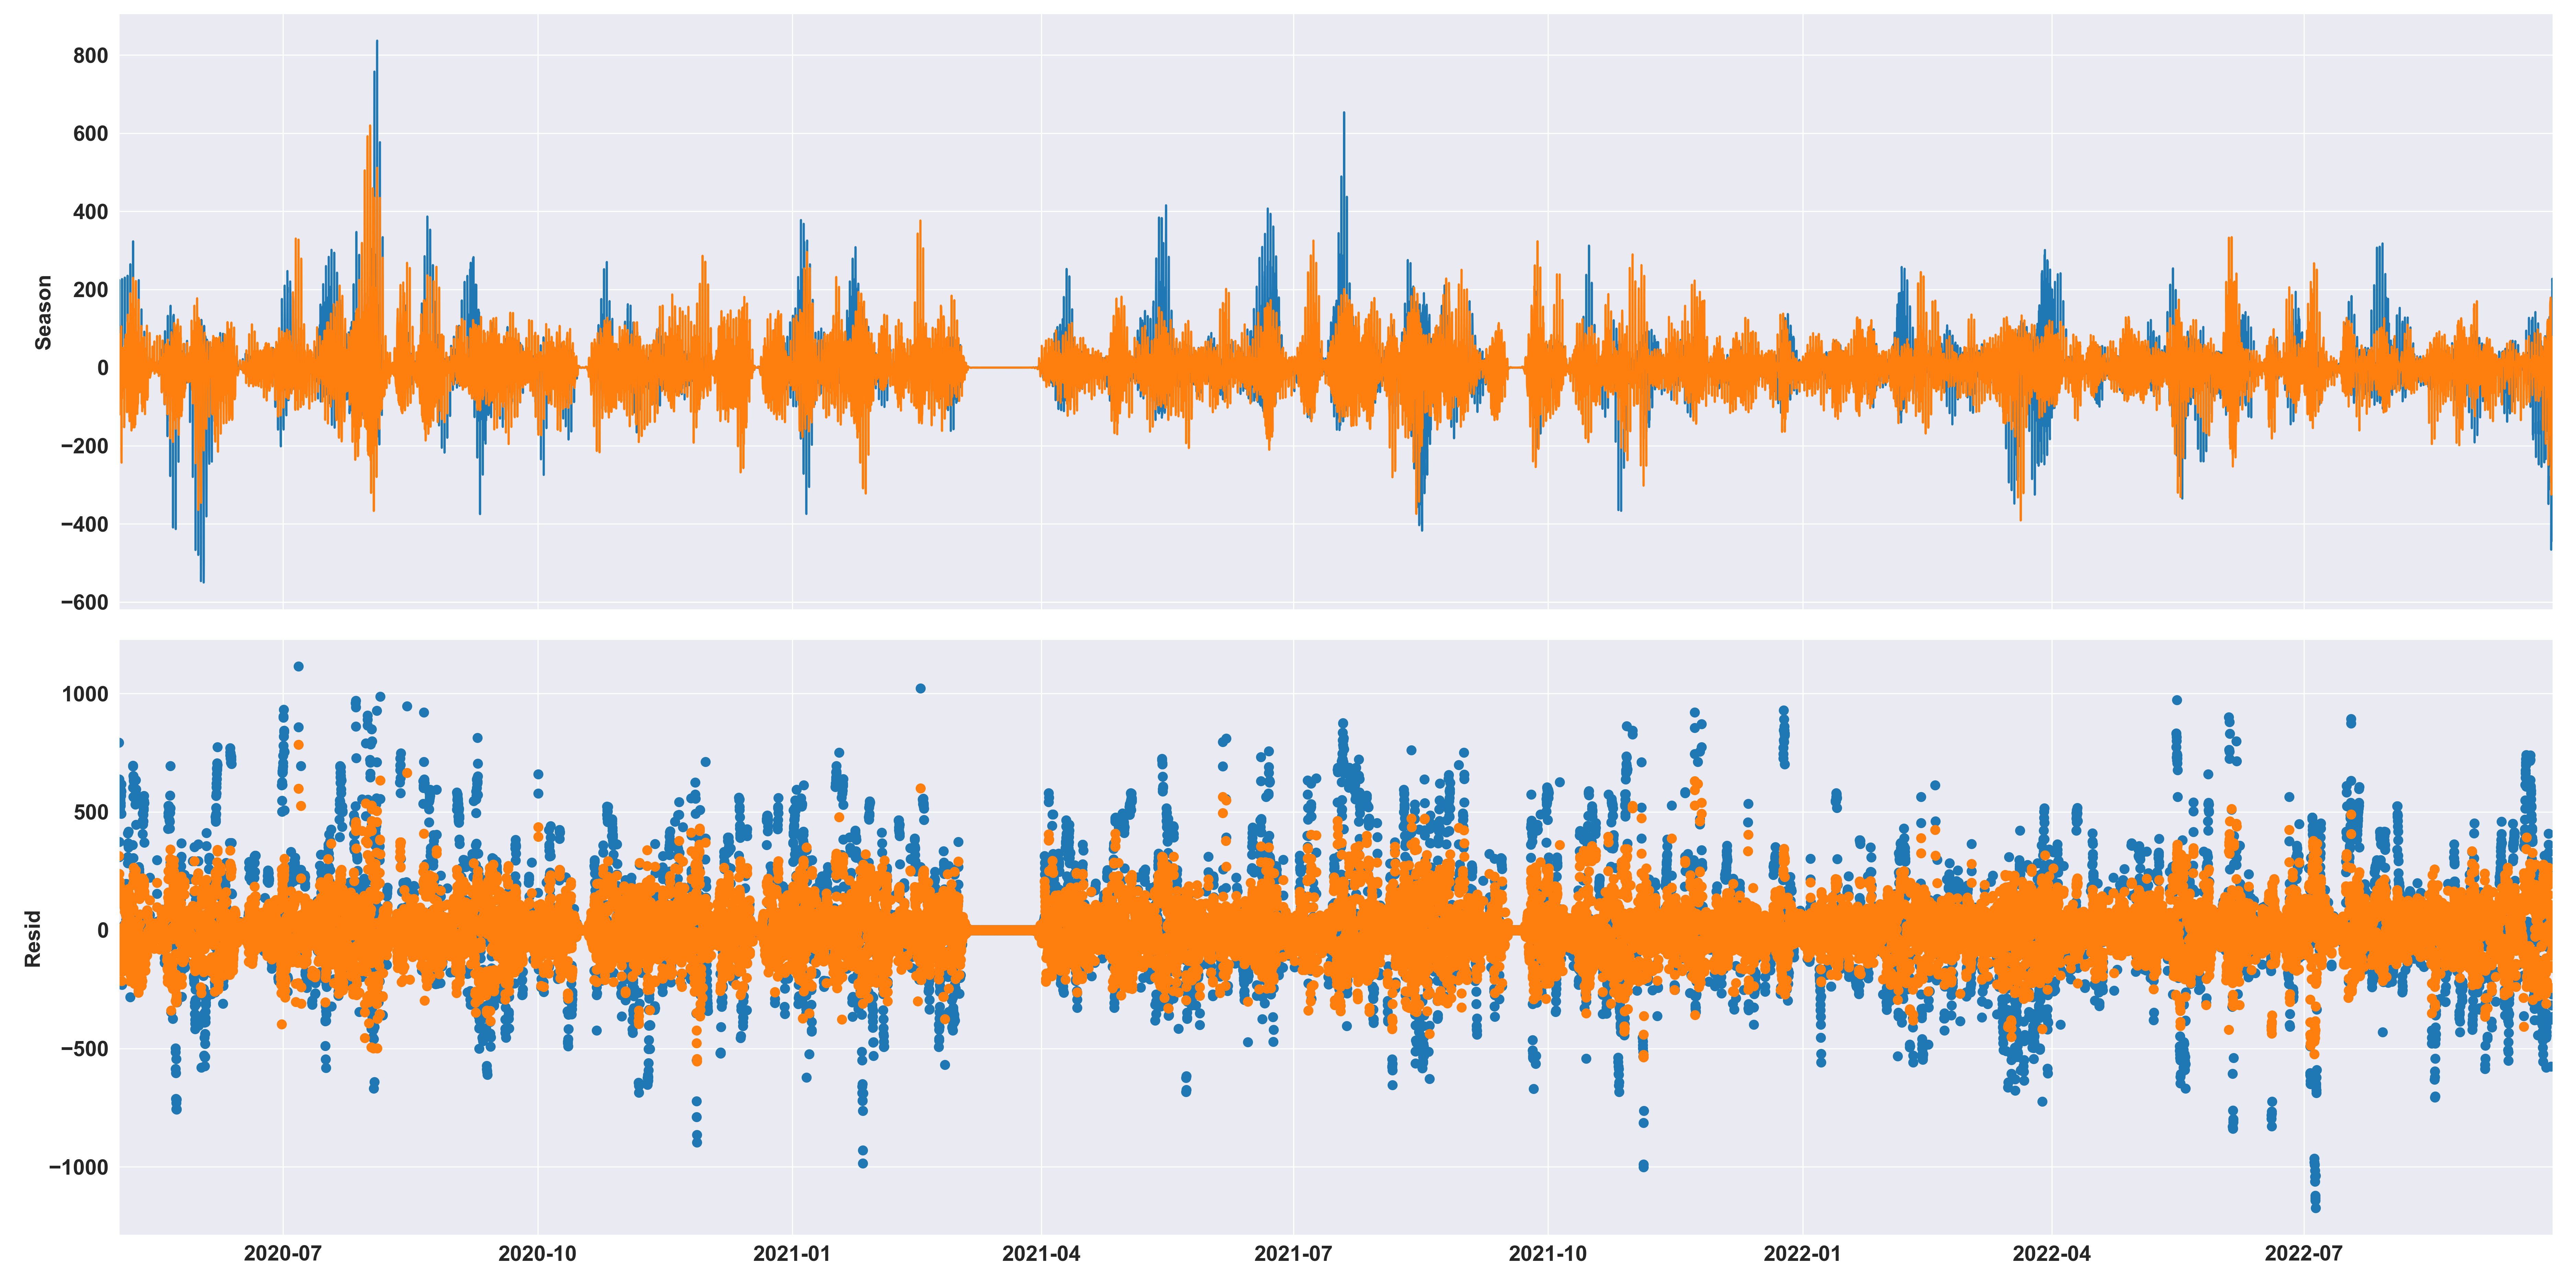
\includegraphics[width=1\textwidth]{Figures/PWR_STL.png}
    \caption{Power STL}
    \label{fig:PWR_STL}
\end{figure}

However, the separate regions of the graph exhibit constant trends during small periods (eg.: July-October).
This potentially can be related to external conditions such as outside temperature depending on the season of the year: the cooling may vary depending on these external conditions, which can lead to either increased or decreased energy consumption.
Moreover, the general increases in energy consumption can be related to the performing of computations, which leads to higher activity of the node and increased power usage, depending on the heaviness of the task.

\begin{figure}[H]
    \centering
    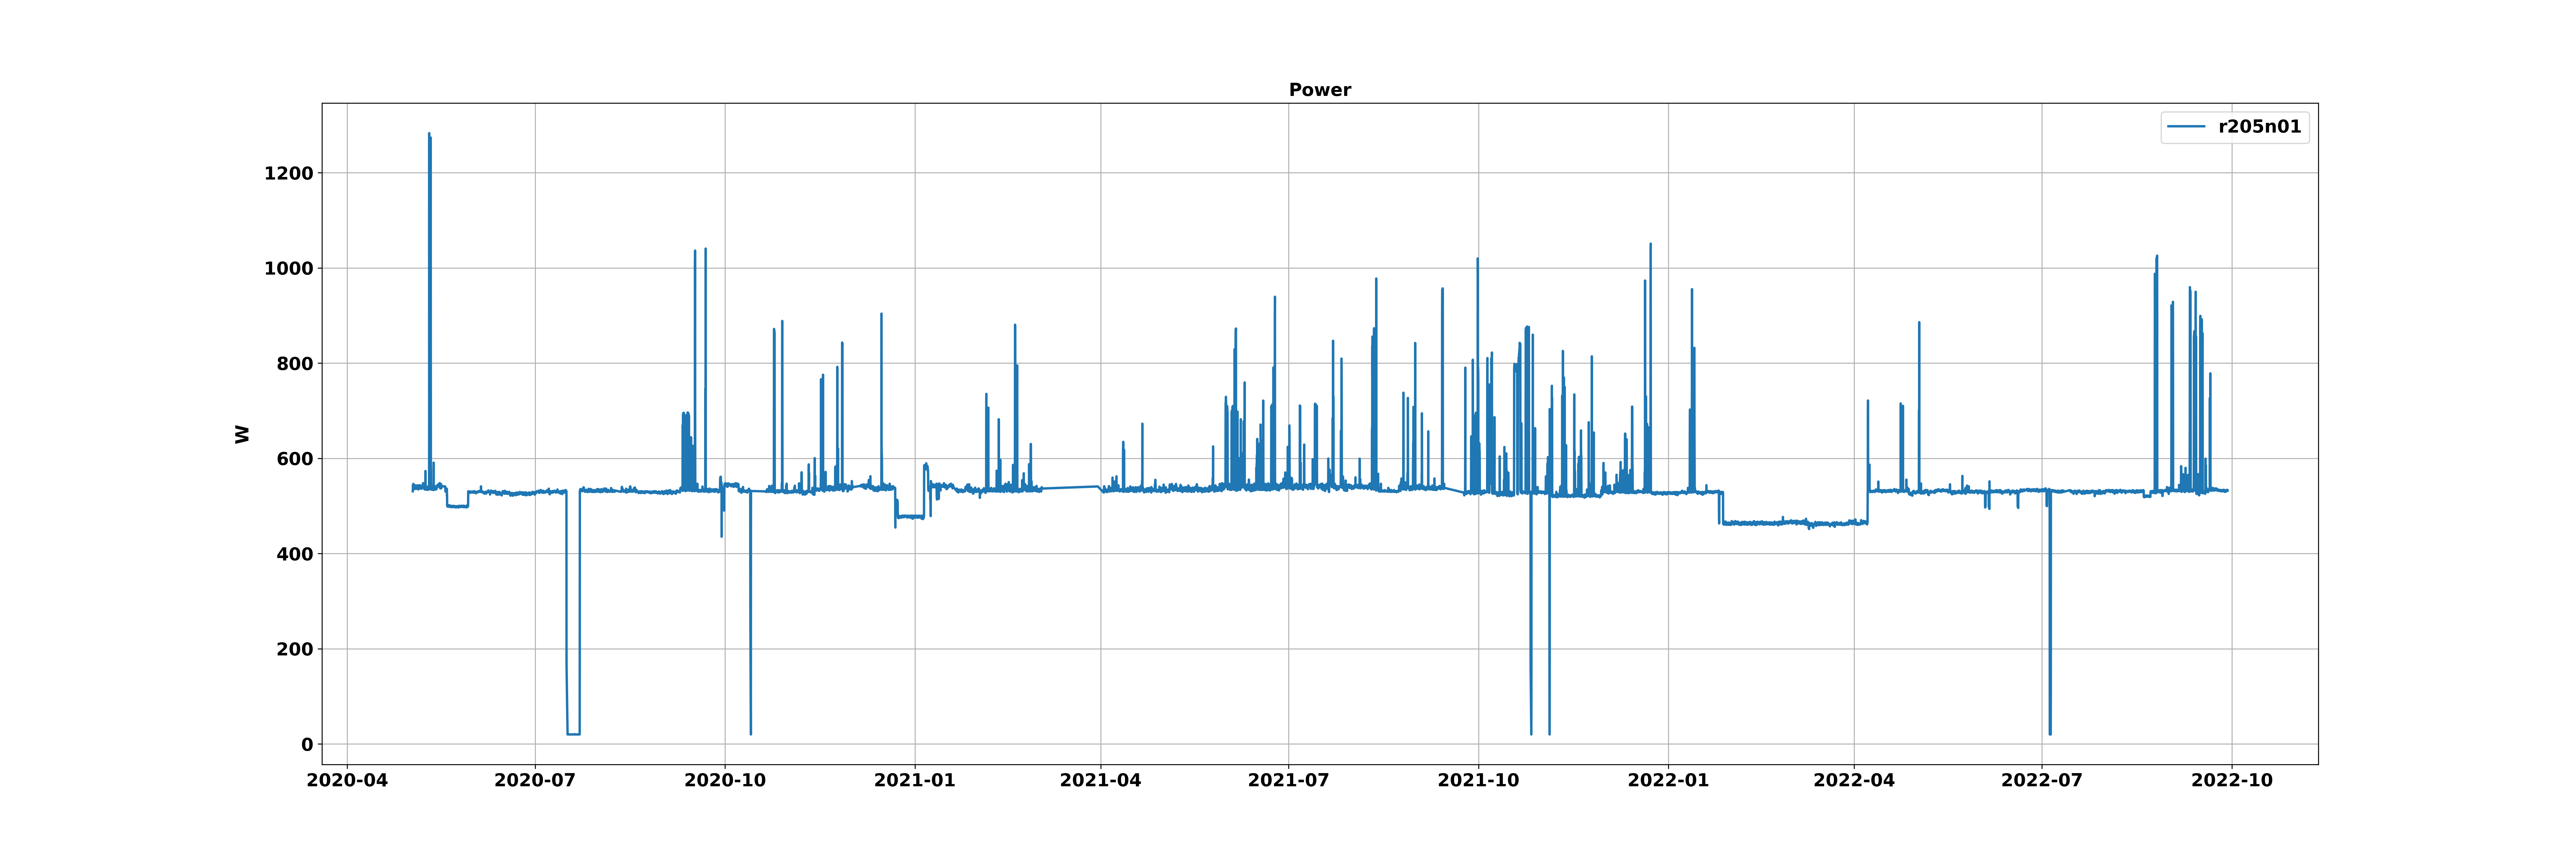
\includegraphics[width=1\textwidth]{Figures/PWR_r205n01.png}
    \caption{Power r205n01}
    \label{fig:PWR_r205n01}
\end{figure}

\begin{figure}[H]
    \centering
    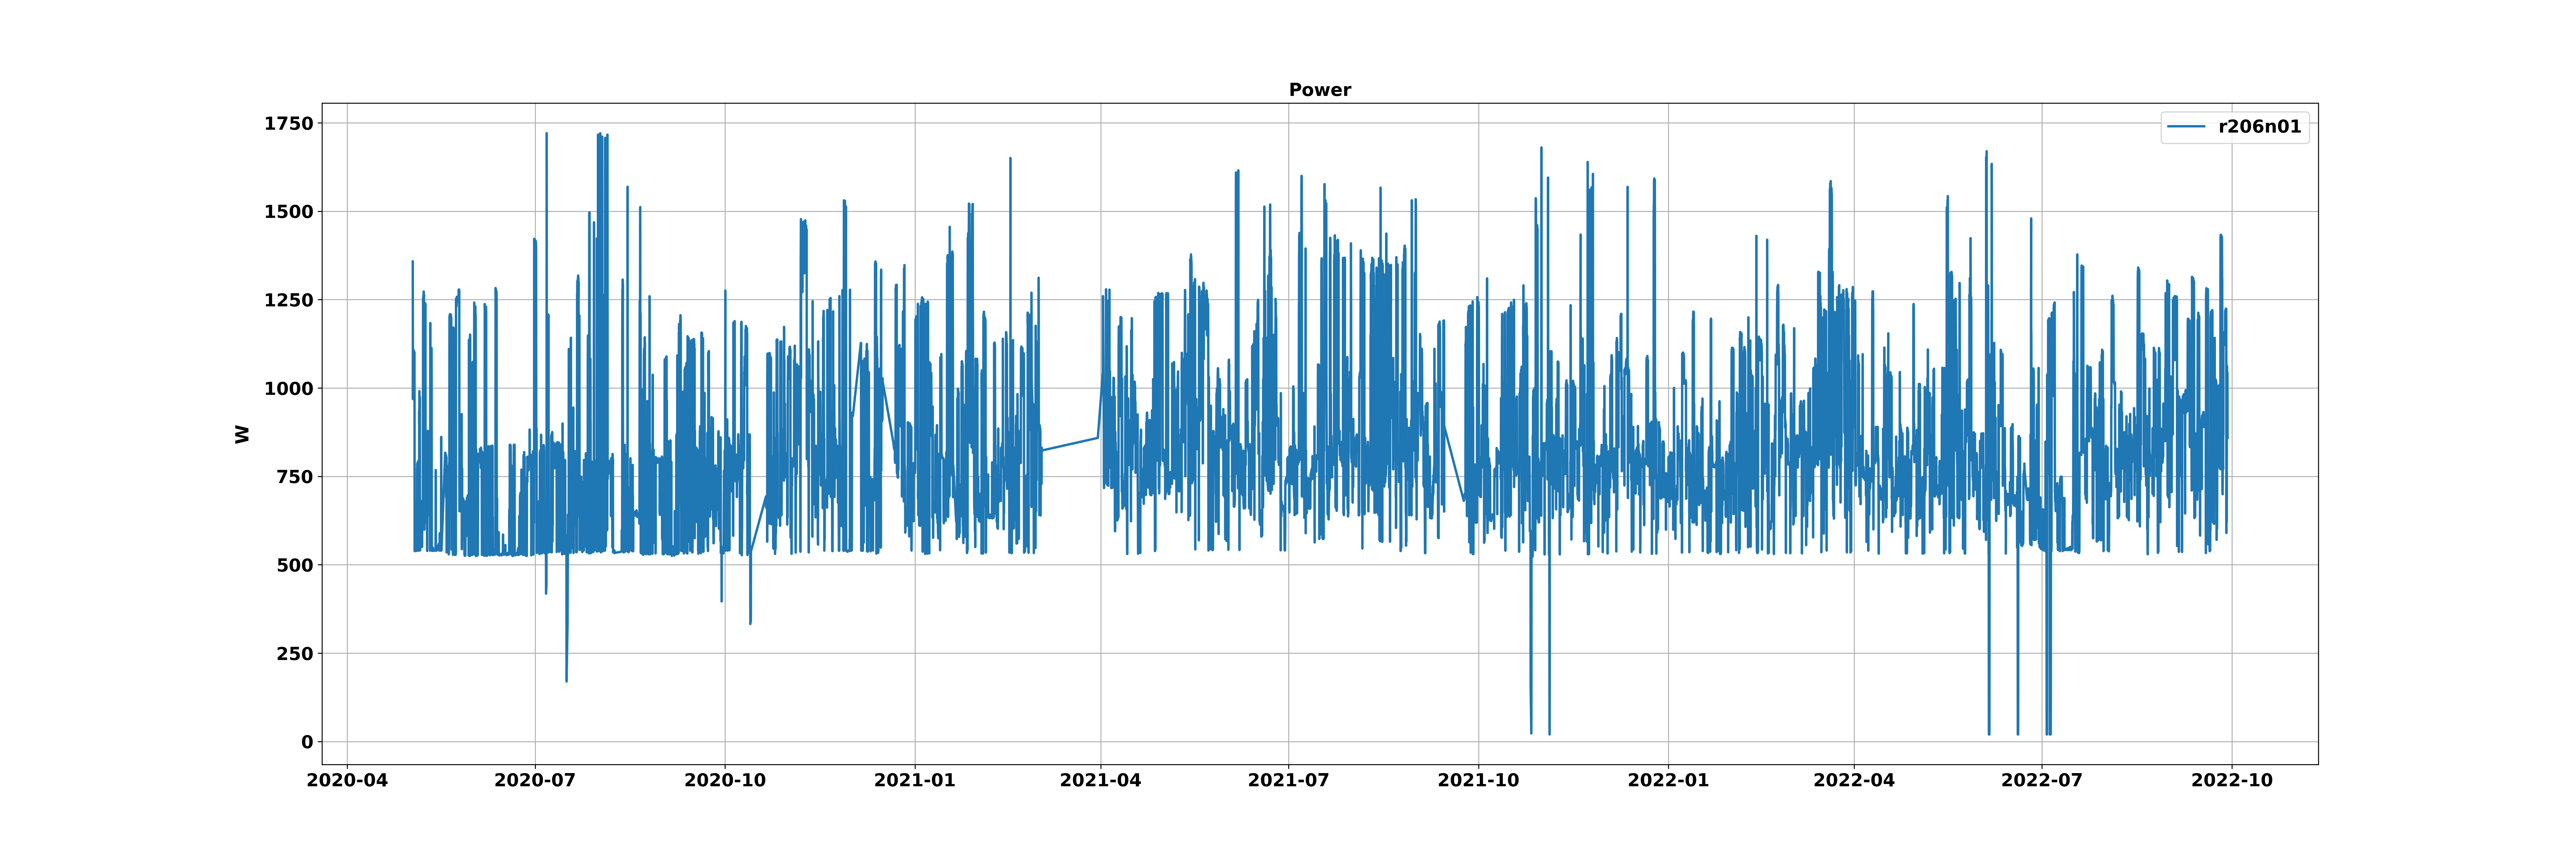
\includegraphics[width=1\textwidth]{Figures/PWR_r206n01.png}
    \caption{Power r206n01}
    \label{fig:PWR_r206n01}
\end{figure}

In terms of power consumption, the comparison of the power data for the r205 and the r206 demonstrates a noticeable difference over the same period, from April 2020 to October 2022.
In both cases the power data shows significant fluctuations: r206 exhibits a higher power usage pattern while r205 shows a more stable and consistent pattern.
It is possible that the first rack may be used for different purposes, such as job submission and task scheduling, resulting in different power consumption patterns compared to other nodes.

\begin{figure}[H]
    \centering
    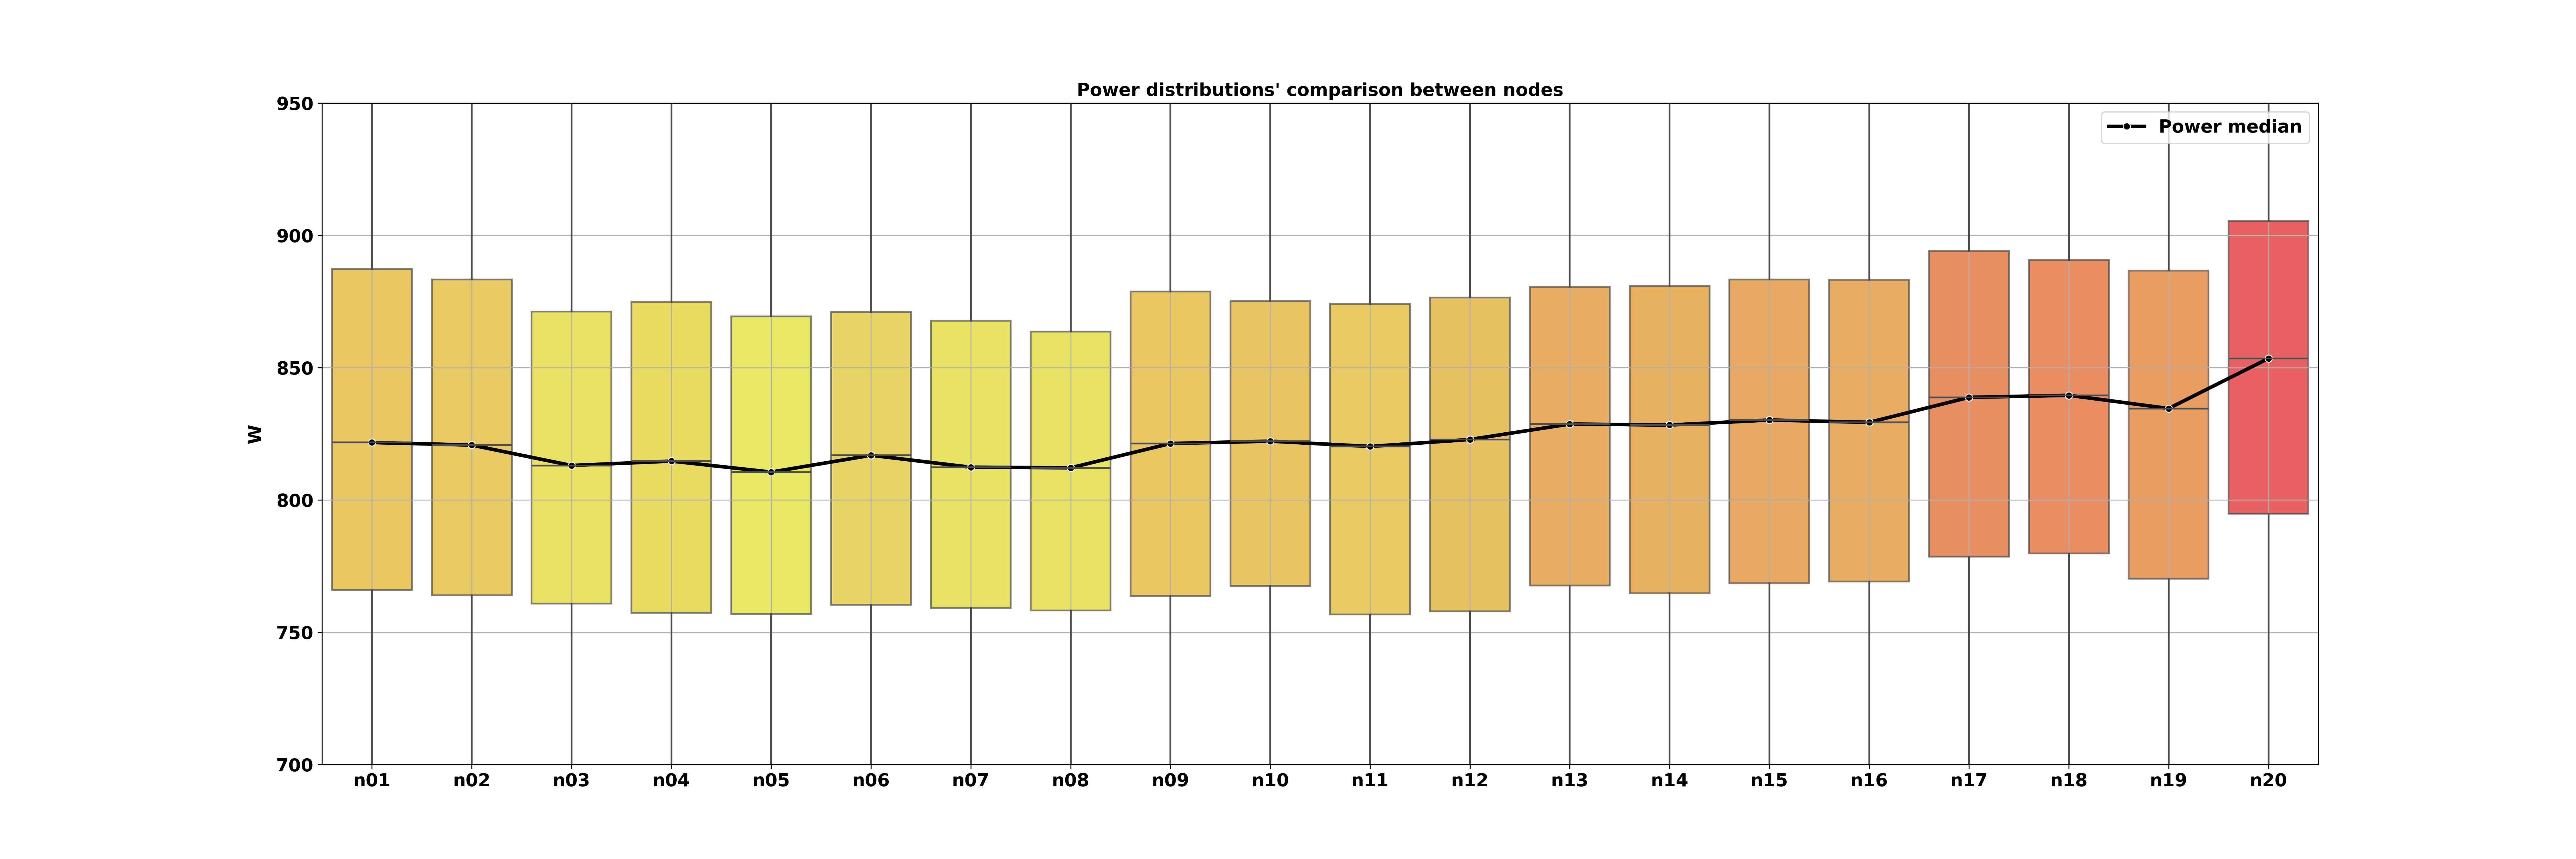
\includegraphics[width=1\textwidth]{Figures/PWR_nodes_boxplot.png}
    \caption{Power distributions comparison between nodes}
    \label{fig:PWR_nodes_boxplot}
\end{figure}

The figure \ref{fig:PWR_nodes_boxplot} provides a comparison of power consumption across 20 different nodes (n01 to n20).
The boxplot represents the data distributions and a line plot shows the median for each node, highlighting the central tendency of power consumption.
Each node shows variability in power consumption, with some nodes having wider variation, indicating more fluctuation in power usage.
Moreover, Nodes located upside (n17 to n20) tend to have higher median power consumption compared to those located on the downside of the rack (n01 to n05). Node n20 shows the highest variability and median power consumption.

\subsection{Temperature of Operation}
Dealing with HPC forces us to take into consideration temperature distribution and the effect it might have on the general performance of the system, given the correlation that exists between power consumption and temperature itself; this correlation can be relatively seen in the following figure \ref{fig:PWR_TEMP}, which is really important for our future considerations:

\begin{figure}[H]
    \centering
    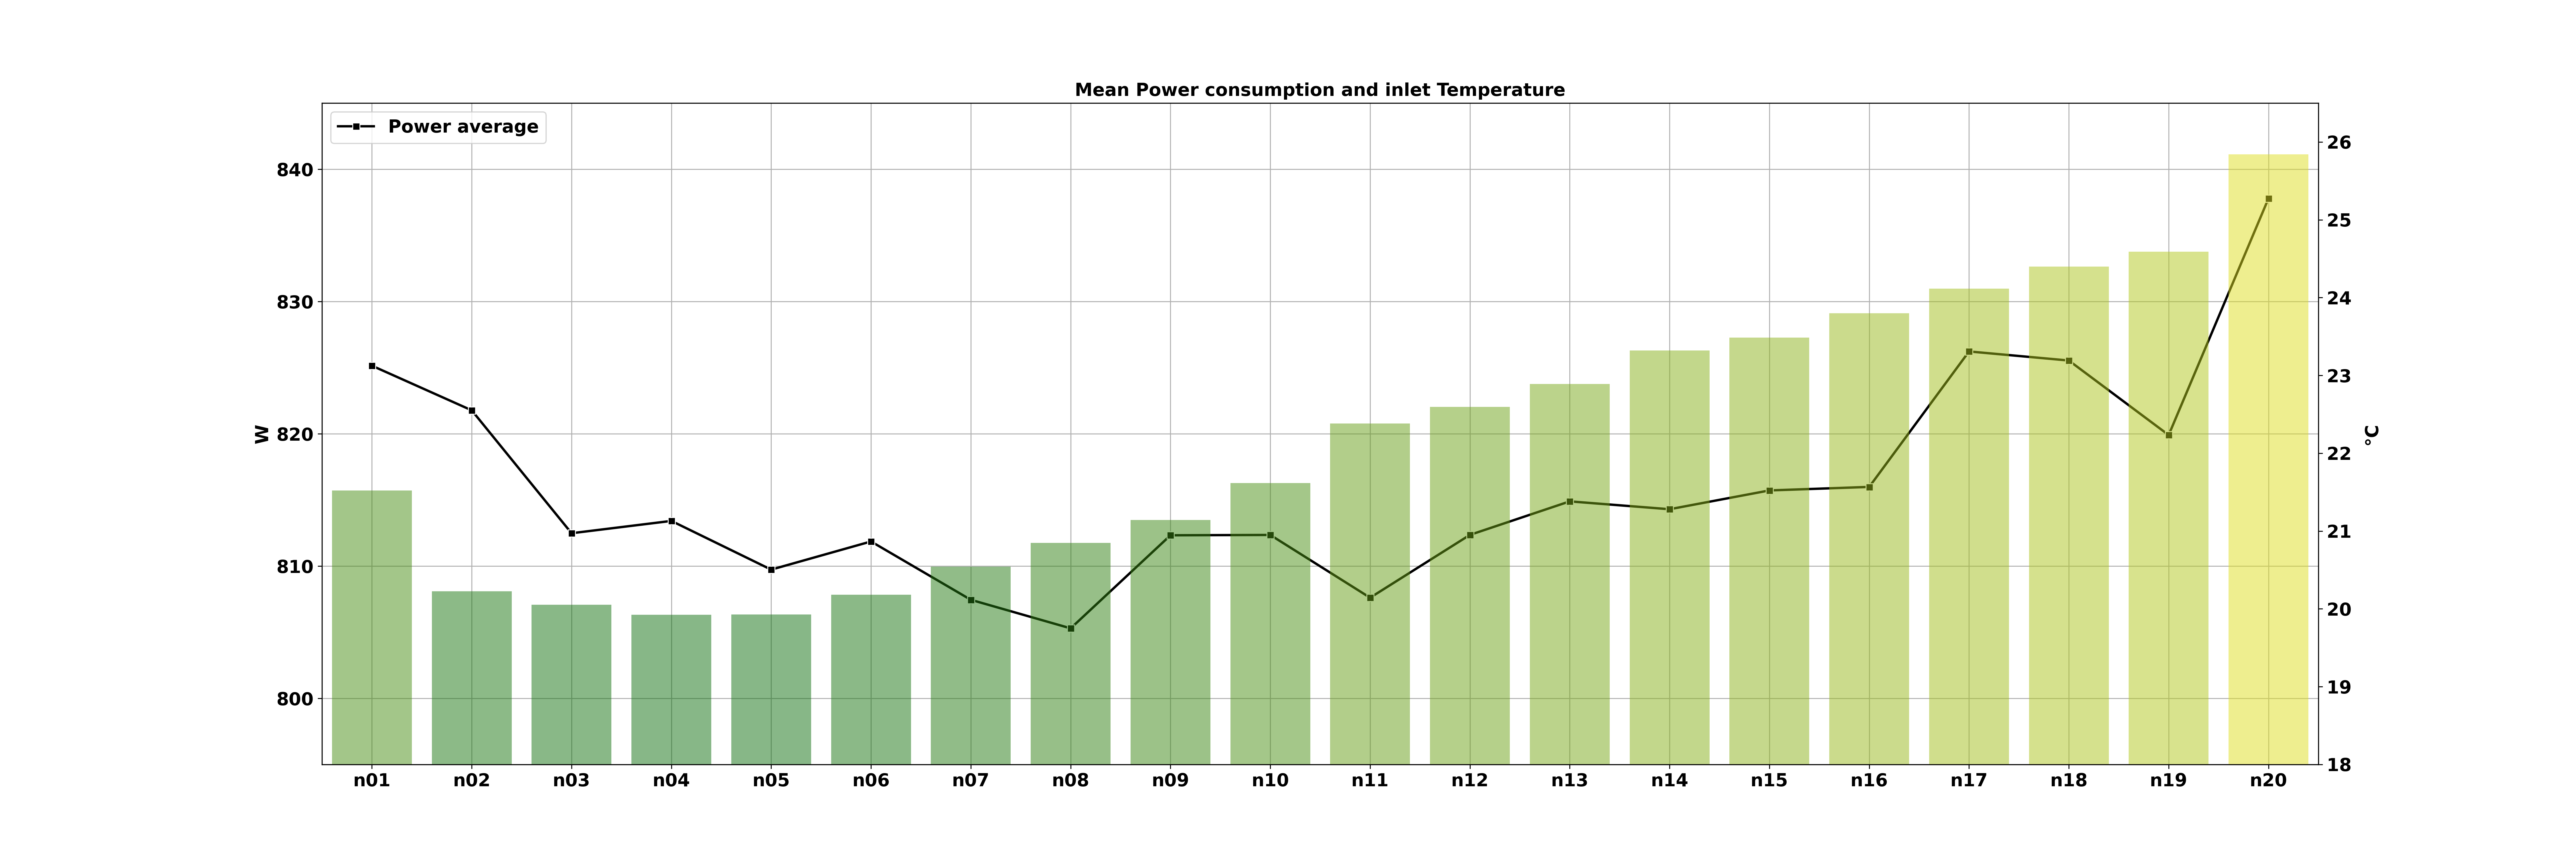
\includegraphics[width=1\textwidth]{Figures/PWR_TEMPin_nodes_mean_plot.png}
    \caption{Power and Temperature observation}
    \label{fig:PWR_TEMP}
\end{figure}

The line trend represents a piece of data we already investigated, the average power that the different nodes consume, while the histogram shows the average inlet temperature of the air flowing into the nodes;
it is clear that the higher nodes tend to receive warmer air with respect to the lower ones, because of heat transfer from bottom to top of the room containing the racks.
Particularly, the plot highlights the tendency of warmer nodes to consume more power.
To further investigate this possible cause of inefficiency we can comment the second figure \ref{fig:TEMP}:

\begin{figure}[H]
    \centering
    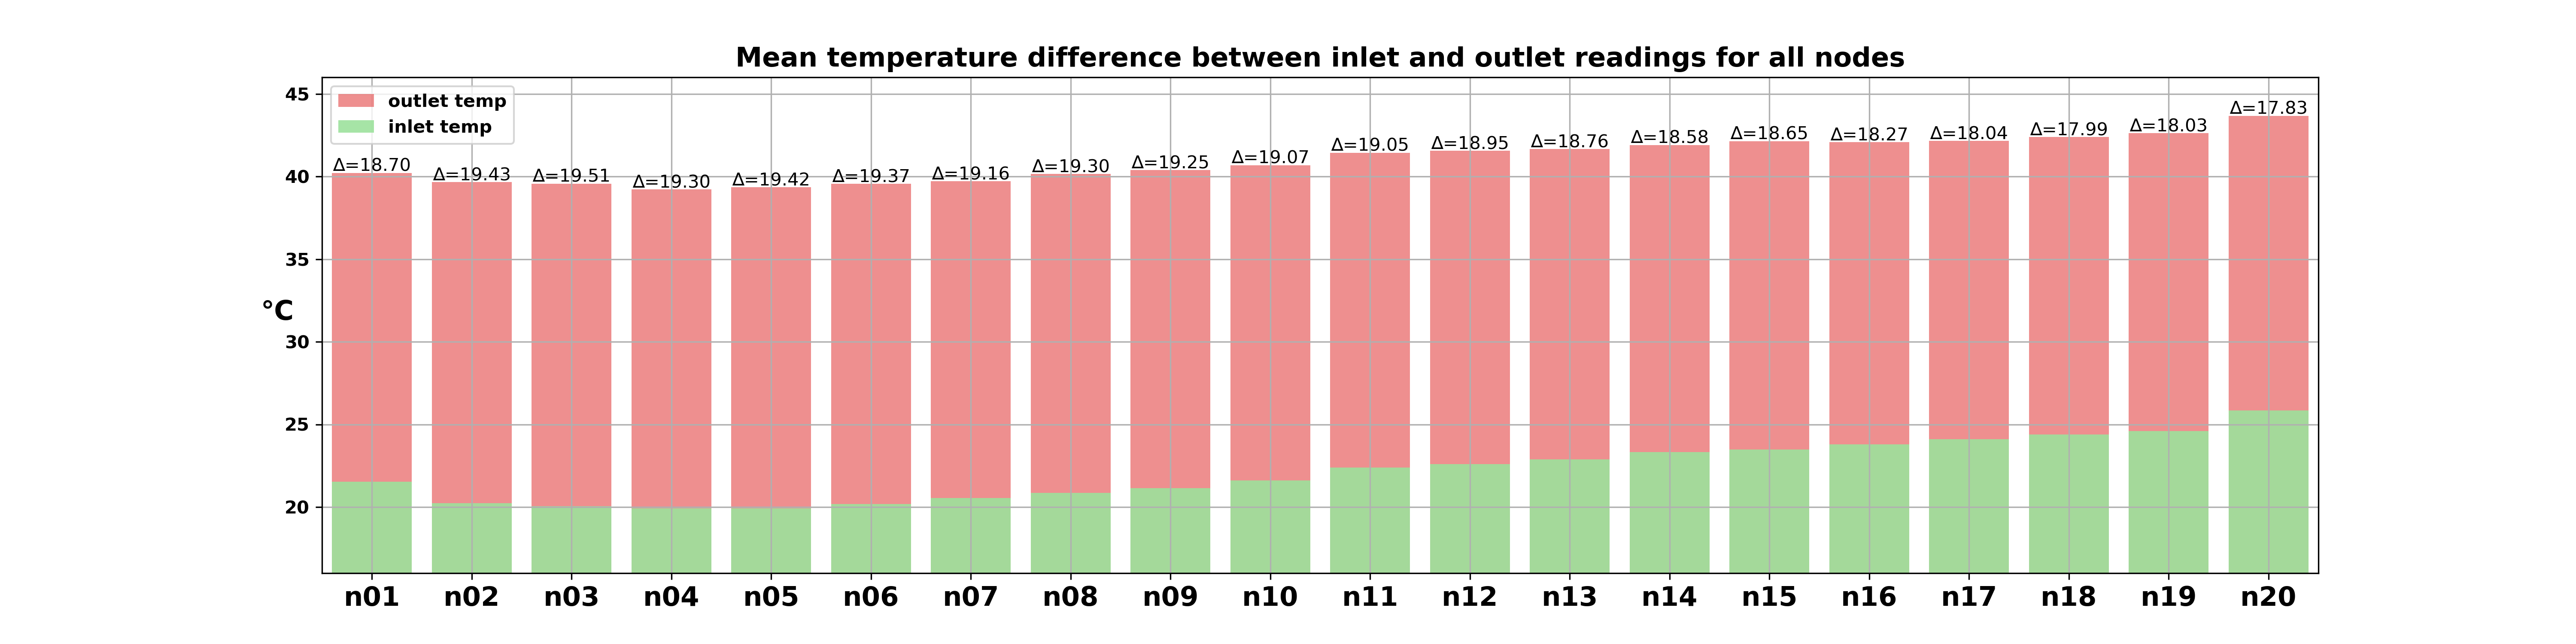
\includegraphics[width=1\textwidth]{Figures/TEMP_difference_plot.png}
    \caption{Inlet and Outlet temperature comparison}
    \label{fig:TEMP}
\end{figure}

The average difference in terms of input and output temperature of similarly positioned nodes doesn’t demonstrate significant difference moving vertically inside the racks.
For this reason we can assume that the distribution of work and tasks throughout the nodes are balanced, given the similar thermal contribution that the nodes produce;
this means that a different approach in the assignment of the computational work (task scheduling) might positively impact the overall power consumption, for example, favoring the lower nodes when possible, due to the temperature distribution impacting it’s performance, which is directly correlated with the power consumption.

\subsection{COP Calculation}
Operational Carbon Footprint (COP) is one of the most important metrics for the goal of our observations since it represents the equivalent $CO_2$ emission generated from a certain amount of energy utilization, expressed in grams of $CO_2$, which represents a fundamental value for green computing analysis.
This quantity is obtained by combining the energy consumption [kWh] with the Carbon Intensity [g$CO_2$/kWh] referred to the geographical area where the energy is used.

\[ COP = E * CI\]

As the COP was calculated (Figure 10) and based on both Energy and CI, it has been demonstrated before that energy doesn’t show any clear predictable pattern, while CI has better predictability, the further work can be focused on developing an enhanced model to predict the COP.

\begin{figure}[H]
    \centering
    \includegraphics[width=1\textwidth]{Figures/COP_Total.png}
    \caption{Total COP}
    \label{fig:COP}
\end{figure}

\subsection{Analysis of Data and Suggestions for Green Computing}
Given these assumptions and hypotheses we wanted to evaluate how much this approach might actually impact on the overall energy consumption; to do so we considered two different cases, always having the same goal: to estimate how much we could have saved in terms of electricity cost and gas emission.
\begin{itemize}
  \item I. With an approximation, we computed our final values using only the average energy per node; then we substituted the upper four nodes’ energy value with the mean value and finally multiplied the obtained energy by the number of racks, taking into consideration that each node is present in all 49 racks.
  \item II. Using the whole 2.5-year distribution of hourly samples for the energy dataset, without the data manipulation, we repeated a similar computation.
\end{itemize}
In both cases, the EUR/MWh cost metric we used has been taken from real data related to Italy \cite{ElectricityCost}, and referred to the cost of wholesale energy directly from the producer; so we need to take into consideration that the actual price per energy tends to be higher for the final customer, like CINECA itself.
\\
Case I returned an approximate yearly saving of around 19.33 MWh, equivalent to 3151.39 €, obtained using the average cost for the energy in that period of time. Case II confirmed the initial result, returning a more accurate 3932.90 € per year, equivalent to 18.62 MWh.
\\
Applying this kind of task management, a total of 9832.24€ could be potentially saved, which is equal to 46.56 MWh in the period of 2.5 years.
But most importantly, this approach might have avoided the production of 25 669.45 kg of equivalent $CO_2$ for the past 21 months.
Comparing these results with the total cost and $CO_2$ emission obtained from the unaltered data within the same period of time, we observe a 16.46\% reduction in gas emission and a significant 18.13\% reduction in the expenses for energy purchase.